\documentclass{standalone}
\usepackage{pgfplots}

\begin{document}
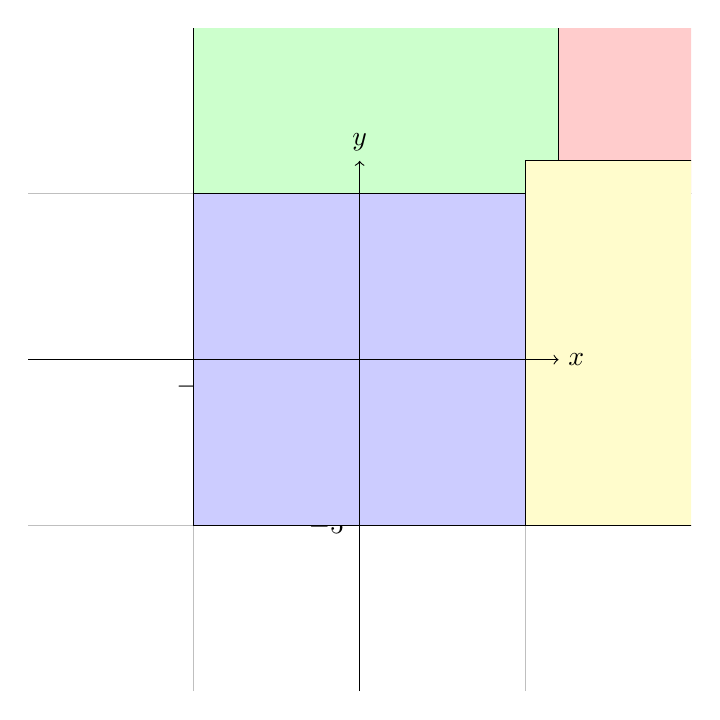
\begin{tikzpicture}
    \begin{axis}[
        axis lines=middle,
        xmin=-10, xmax=10,
        ymin=-10, ymax=10,
        xtick={-5,0,5},
        ytick={-5,0,5},
        grid=major,
        width=10cm,
        height=10cm,
        enlargelimits=false,
    ]
    
    % Define the coordinates for the boxes
    \coordinate (A) at (axis cs:-5,-5);
    \coordinate (B) at (axis cs:5,5);
    \coordinate (C) at (axis cs:-5,5);
    \coordinate (D) at (axis cs:5,-5);
    
    % Draw the boxes
    \draw[fill=blue!20] (A) rectangle ++(1,1);
    \draw[fill=red!20] (B) rectangle ++(1,1);
    \draw[fill=green!20] (C) rectangle ++(1,1);
    \draw[fill=yellow!20] (D) rectangle ++(1,1);
    
    % Draw the coordinate system for reference
    \draw[->] (-6,0) -- (6,0) node[right] {$x$};
    \draw[->] (0,-6) -- (0,6) node[above] {$y$};
    
    \end{axis}
\end{tikzpicture}
\end{document}